% Created 2016-04-28 tor 16:50
% Intended LaTeX compiler: pdflatex
\documentclass{scrartcl}
\usepackage[utf8]{inputenc}
\usepackage[T1]{fontenc}
\usepackage{graphicx}
\usepackage{grffile}
\usepackage{longtable}
\usepackage{wrapfig}
\usepackage{rotating}
\usepackage[normalem]{ulem}
\usepackage{amsmath}
\usepackage{textcomp}
\usepackage{amssymb}
\usepackage{capt-of}
\usepackage{hyperref}
\usepackage{khpreamble}
\newcommand{\tustin}{\frac{2}{h}\frac{z-1}{z+1}}
\author{Kjartan Halvorsen}
\date{2015-11-17}
\title{Computerized control - partial exam 3 (dummy) - modified from Fall 2015}
\hypersetup{
 pdfauthor={Kjartan Halvorsen},
 pdftitle={Computerized control - partial exam 3 (dummy) - modified from Fall 2015},
 pdfkeywords={},
 pdfsubject={},
 pdfcreator={Emacs 24.5.1 (Org mode 8.3.4)}, 
 pdflang={English}}
\begin{document}

\maketitle
In the last lecture we looked at a state-space model of the harmonic oscillator with state variables corresponding to the position and velocity of the oscillating mass. If the frequency of the oscillations is \(\omega=1\) and we sample the system with zero-order-hold  with a sampling period \(h\) such that \(\omega h = 0.4\) we obtain the sampled system
\begin{equation}
\begin{split}
x(k+1) &= \bbm 0.92 & 0.39\\ -0.39 & 0.92 \ebm x(k) + \bbm 0.079\\0.39 \ebm u(k)\\
y(k)  &= \bbm 1 & 0 \ebm x(k)
\end{split}
\label{eq:ss}
\end{equation}

\section*{Problem 1}
\label{sec:orgheadline1}
Verify that the pulse-transfer function is 
\begin{equation}
H(z) = \frac{0.079(z+1)}{z^2 - 1.84z + 1.0} = \frac{0.079(z+1)}{(z-0.92)^2 + 0.15}.
\end{equation}
Plot the zeros and poles of the discrete-time system \textbf{and} of the continuous-time system in the complex plane in figure \ref{fig:complex-plane}.
\begin{figure}[h]
\begin{center}
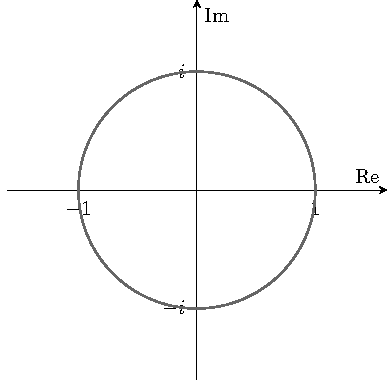
\includegraphics[]{complex-plane}
\caption{Problem 1: Plot the poles and zeros of the system (both discrete-time and continuous-time).}
\label{fig:complex-plane}
\end{center}
\end{figure}

\section*{Problem 2}
\label{sec:orgheadline2}
A PD-regulator for the continuous-time harmonic oscillator has been designed. It is sampled using Tustin's formula to give the discrete-time controller
\begin{equation}
F(z) = \frac{5z-3.4}{z+0.6}.
\end{equation}
The system is controlled by error-feedback, according to figure \ref{fig:error-feedback}. Calculate the pulse-transfer function for the closed-loop system from \(u_c\) to \(y\).
\begin{figure}[h]
\begin{center}
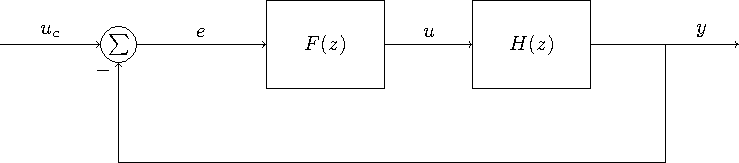
\includegraphics[]{error-feedback}
\caption{Problem 2: Error feedback with PD-control.}
\label{fig:error-feedback}
\end{center}
\end{figure}

\section*{Problem 3}
\label{sec:orgheadline3}
Assume that the requirements on the properties of the discrete-time closed-loop system is that it should have two complex-conjugated poles at 
\begin{equation}
0.3 \pm 0.3i
\end{equation}
In addition, there should be an observer pole in the origin (deadbeat observer). Hence, the desired closed-loop characteristic polynomial is
\begin{equation}
A_{cl} = A_cA_o = (z-0.3-0.3i)(z-0.3+0.3i)z = z^3 - 0.6z^2 + 0.18z, 
\end{equation}
with observer polynomial \(A_o=z\).
Design a RST-controller (see figure \ref{fig:rst}) that gives the desired closed-loop characteristic polynomial, and such that the pulse-transfer function from \(u_c\) to \(y\) has static gain equal to one (\(G_c(1) = 1)\). 
\begin{figure}[h]
\begin{center}
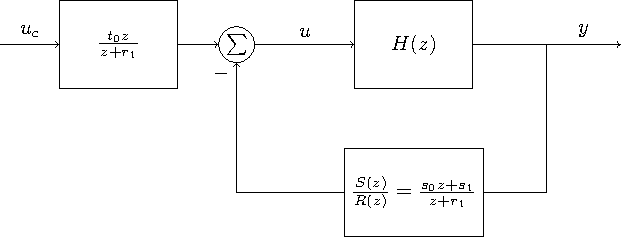
\includegraphics[]{rst}
\caption{Problem 4: RST-controller.}
\label{fig:rst}
\end{center}
\end{figure}
It is sufficient to set up the linear system of equations to solve for \(s_0\), \(s_1\) and \(r_1\).

\section*{Problem 4}
\label{sec:orgheadline4}
Assume that both the position and the velocity of the moving mass are measured. We thus have a measurement of the state \(x(k)\) available, and we can use these two measurements to implement state feedback control according to the control law
\begin{equation}
u(k) = -l_1x_1(k) - l_2x_2(k) = -Lx(k).
\end{equation}
Determine the state feedback gain \(L\) such that the closed-loop system has characteristic polynomial
\begin{equation}
z^2 - 0.6z + 0.18.
\end{equation}
It is sufficient to set up the linear system of equations to solve for \(l_1\) and \(l_2\). 

\section*{Solutions}
\label{sec:orgheadline9}
\subsection*{Problem 1}
\label{sec:orgheadline5}
The pulse-transfer function is given by
\begin{equation*}
\begin{split}
H(z) &= C\left(zI - \Phi\right)\inv \Gamma\\
     &= \bbm 1 & 0 \ebm \bbm z-0.92 & -0.39\\0.39 & z-0.92 \ebm\inv \bbm 0.079\\0.39 \ebm\\
     &= \frac{1}{(z-0.92)^2 + 0.39^2}\bbm 1 & 0 \ebm \bbm z-0.92 & 0.39\\-0.39 & z-0.92 \ebm \bbm 0.079\\0.39\ebm \\
     &= \frac{0.079(z+1)}{(z-0.92)^2 + 0.15}.
\end{split}
\end{equation*}
\begin{center}
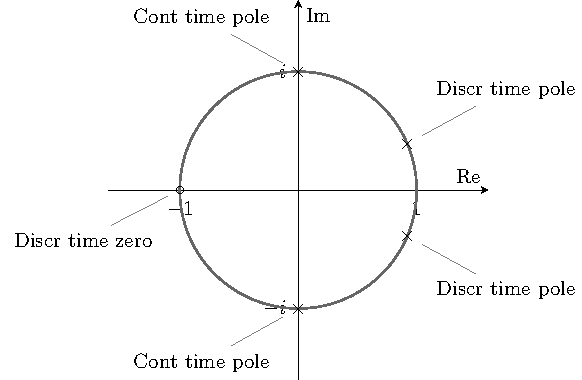
\includegraphics[]{complex-plane-sol}
\end{center}
\subsection*{Problem 2}
\label{sec:orgheadline6}
Write the pulse-transfer function of the controller as 
\[ F(z) = \frac{B_f(z)}{A_f(z)}, \] and the plant as
\[ H(z) = \frac{B(z)}{A(z)}. \]
The pulse transfer function of the closed-loop system is given by
\begin{equation*}
\begin{split}
H_c(z) &= \frac{H(z)F(z)}{1 + H(z)F(z)} = \frac{\frac{B(z)}{A(z)}\frac{B_f(z)}{A_f(z)}}{1 + \frac{B(z)}{A(z)}\frac{B_f(z)}{A_f(z)}}\\
       &= \frac{B(z)B_f(z)}{A(z)A_f(z) + B(z)B_f(z)} = \frac{0.079(z+1)(5z-3.4)}{(z^2 -1.84z + 1)(z+0.6) +  0.079(z+1)(5z-3.4)}\\
       &= \frac{0.395(z+1)(z-0.68)}{z^3 -1.24z^2 -0.104z + 0.6 + 0.395(z^2 + 0.32z-0.68)}\\
       &= \frac{0.395(z+1)(z-0.68)}{z^3 -0.845z^2 + 0.0224z + 0.3314}
\end{split}
\end{equation*}
\subsection*{Problem 3}
\label{sec:orgheadline7}
With a first order controller 
\[ \frac{S(z)}{R(z)} = \frac{s_0z + s_1}{z + r_z}, \]
the diophantine equation \(AR + BS = A_{cl}\) becomes
\begin{equation*}
\begin{split}
(z^2 - 1.84z + 1)(z + r_1) + 0.079(z+1)(s_0z+s_1) &= z^3 - 0.6z^2 + 1.18z\\
z^3 + (-1.84 + r_1 + 0.079s_0)z^2 + (1 - 1.84r_1 + 0.079(s_0 + s_1))z + r_1 + 0.079s_1 &= z^3 - 0.6z^2 + 1.18z
\end{split}
\end{equation*}
which leads to the following linear equation in the controller parameters \(s_0\), \(s_1\) and \(r_1\):
\begin{equation*}
\bbm 0.079 & 0 & 1\\ 0.079 & 0.079 & -1.84\\ 0 & 0.079 & 1\ebm \bbm s_0\\s_1\\r_1\ebm = 
\bbm -0.6+1.84\\0.18-1\\0\ebm
\end{equation*}
with solution
\[ \bbm s_0\\s_1\\r_1\ebm = \bbm  8.90\\-6.80\\0.54\ebm. \]
\subsection*{Problem 4}
\label{sec:orgheadline8}
The desired closed-loop characteristic equation is 
\[ z^2 - 0.6z + 0.18. \]
With the state feedback 
\[ u(k) = -Lx(k) = - \bbm l_1 & l_2 \ebm x(k) \]
the closed-loop characteristic equation becomes
\[ \det \left( zI - \Phi + \Gamma L \right), \]
where
\[ \Gamma L = \bbm 0.079\\0.39 \ebm \bbm l_1 & l_2 \ebm = \bbm 0.079l_1 & 0.079l_2\\ 0.39l_1 & 0.39l_2 \ebm. \]
We get
\begin{equation*}
\begin{split}
\det  \left( zI - \Phi + \Gamma L \right) &= \det \left( \bbm z & 0\\ 0 & z \ebm - \bbm 0.92 & 0.39\\ -0.39 & 0.92 \ebm  +\bbm 0.079l_1 & 0.079l_2\\ 0.39l_1 & 0.39l_2 \ebm \right)\\
&= \det \bbm z-0.92 + 0.079l_1 & -0.39+0.079l_2\\0.39+0.39l_1 & z -0.92 + 0.39l_2 \ebm \\
&= ( z-0.92 + 0.079l_1 ) (z -0.92 + 0.39l_2) - ( -0.39+0.079l_2)(0.39+0.39l_1)\\
& = z^2 + (-1.84+0.079l_1 + 0.39l_2)z + 1-0.39l_2 + 0.079l_2.
\end{split}
\end{equation*}
Comparing this to the desired characteristic polynomial gives the system of equations
\begin{equation*}
\bbm 0.079 & 0.39\\0.079 &- 0.39\ebm \bbm l_1\\l_2 \ebm = \bbm -0.6 + 1.84\\ 0.18-1 \ebm
\end{equation*}
with solution
\[ \bbm l_1\\l_2 \ebm = \bbm 2.65\\2.64\ebm. \]
\end{document}
